\documentclass{beamer}

\usepackage{amsmath}
\usepackage{amssymb}
\usepackage{amsthm}
\usepackage{tikz}
\usepackage{pgfplots}
\usepackage{graphicx}
\graphicspath{ {./img/} }

\usetheme{default}

\title{Inverting Vickrey}
\date{}

\begin{document}

\begin{frame}{\titlepage}
  
\end{frame}

\begin{frame}
  \frametitle{The cost function}
  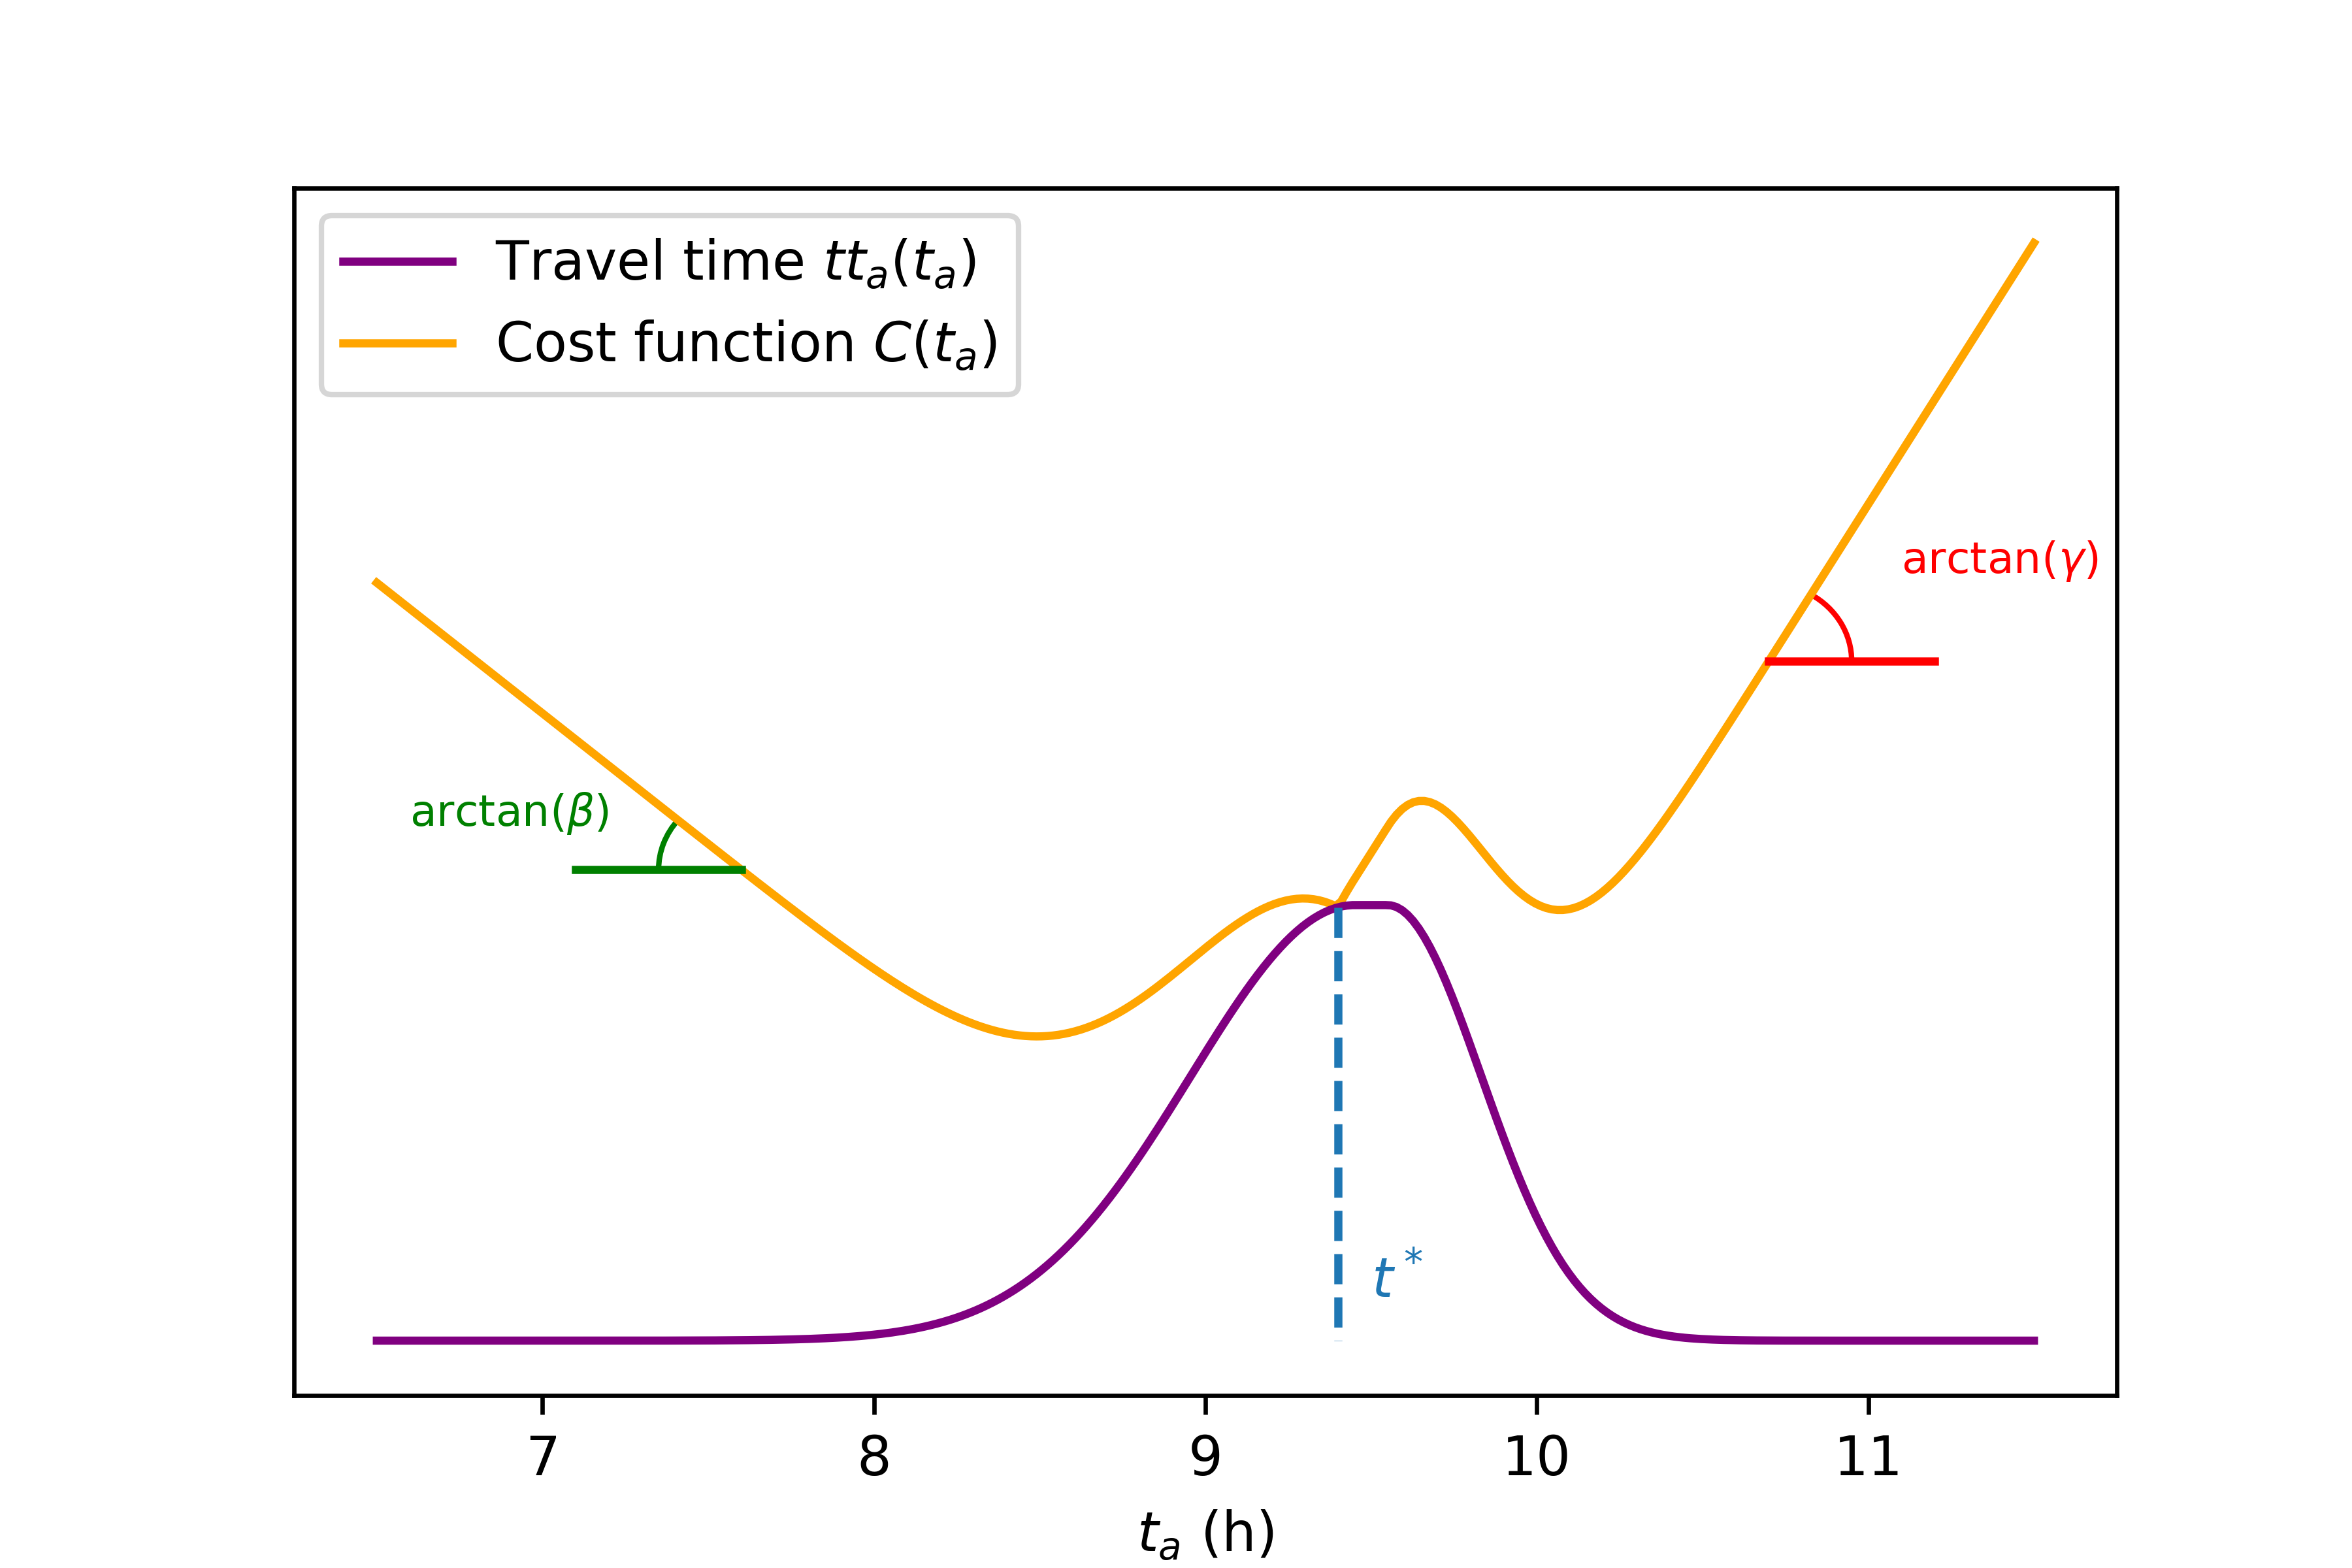
\includegraphics[width=\textwidth]{cost}
\end{frame}

\begin{frame}{The setting}
  \only<-2>{
    We are assuming the cost function to be
    \begin{equation}
      \label{eq:cost}
      C(t_d) = \alpha tt(t_d) + \beta[t^*-t_d-tt(t_d)]^+ + \gamma[t_d+tt(t_d)-t^*]^+ 
    \end{equation}
  }
    \only<1>{
      where
      \begin{itemize}
      \item \(t^*\) is the desired arrival time
      \item \(\alpha\) is the value of time spent travelling
      \item \(\beta\) is the value of time spent waiting there
      \item \(\gamma\) is the value of time arriving late
      \item \(tt(t_d)\) is the expected (exogenous) travel time if leaving at time \(t_d\).
      \item \([x]^+ = \max(0, x)\)
      \end{itemize}
    }
    \only<2>{
      Without loss of generality, we can assume \(\alpha = 1\).

      Moreover, by defining the arrival time
      \begin{equation*}
        t_a = t_d + tt(t_d)
      \end{equation*}
      equation \eqref{eq:cost} becomes
    }
    \uncover<2->{
      \begin{equation}
        \label{eq:cost_ta}
        C(t_a) = tt_a(t_a) + \beta[t^*-t_a]^+ + \gamma[t_a-t^*]^+
      \end{equation}
    }
    \uncover<3>{
      We now assume the parameters \(\beta\), \(\gamma\) and the desired arrival times \(t^*\) to be normally distributed:
      \begin{itemize}
      \item \(\beta \sim \mathcal{N}(\mu_\beta, \sigma)\)
      \item \(\gamma \sim \mathcal{N}(\mu_\gamma, \sigma)\)
      \item \(t^* \sim \mathcal{N}(\mu_t, \sigma_t)\)
      \end{itemize}
    }
\end{frame}

\begin{frame}{Optimal arrival time samples}
  
  \begin{columns}
    \column{.4\linewidth}
      Drawing samples from these distributions, using a typical travel time function \(tt(t_a)\), the optima will be (in general) distributed as shown in the plot,
      where the green and red zones roughly correspond to, respectively, early and late arrivals.

    \column{.6\linewidth}
    \centering
      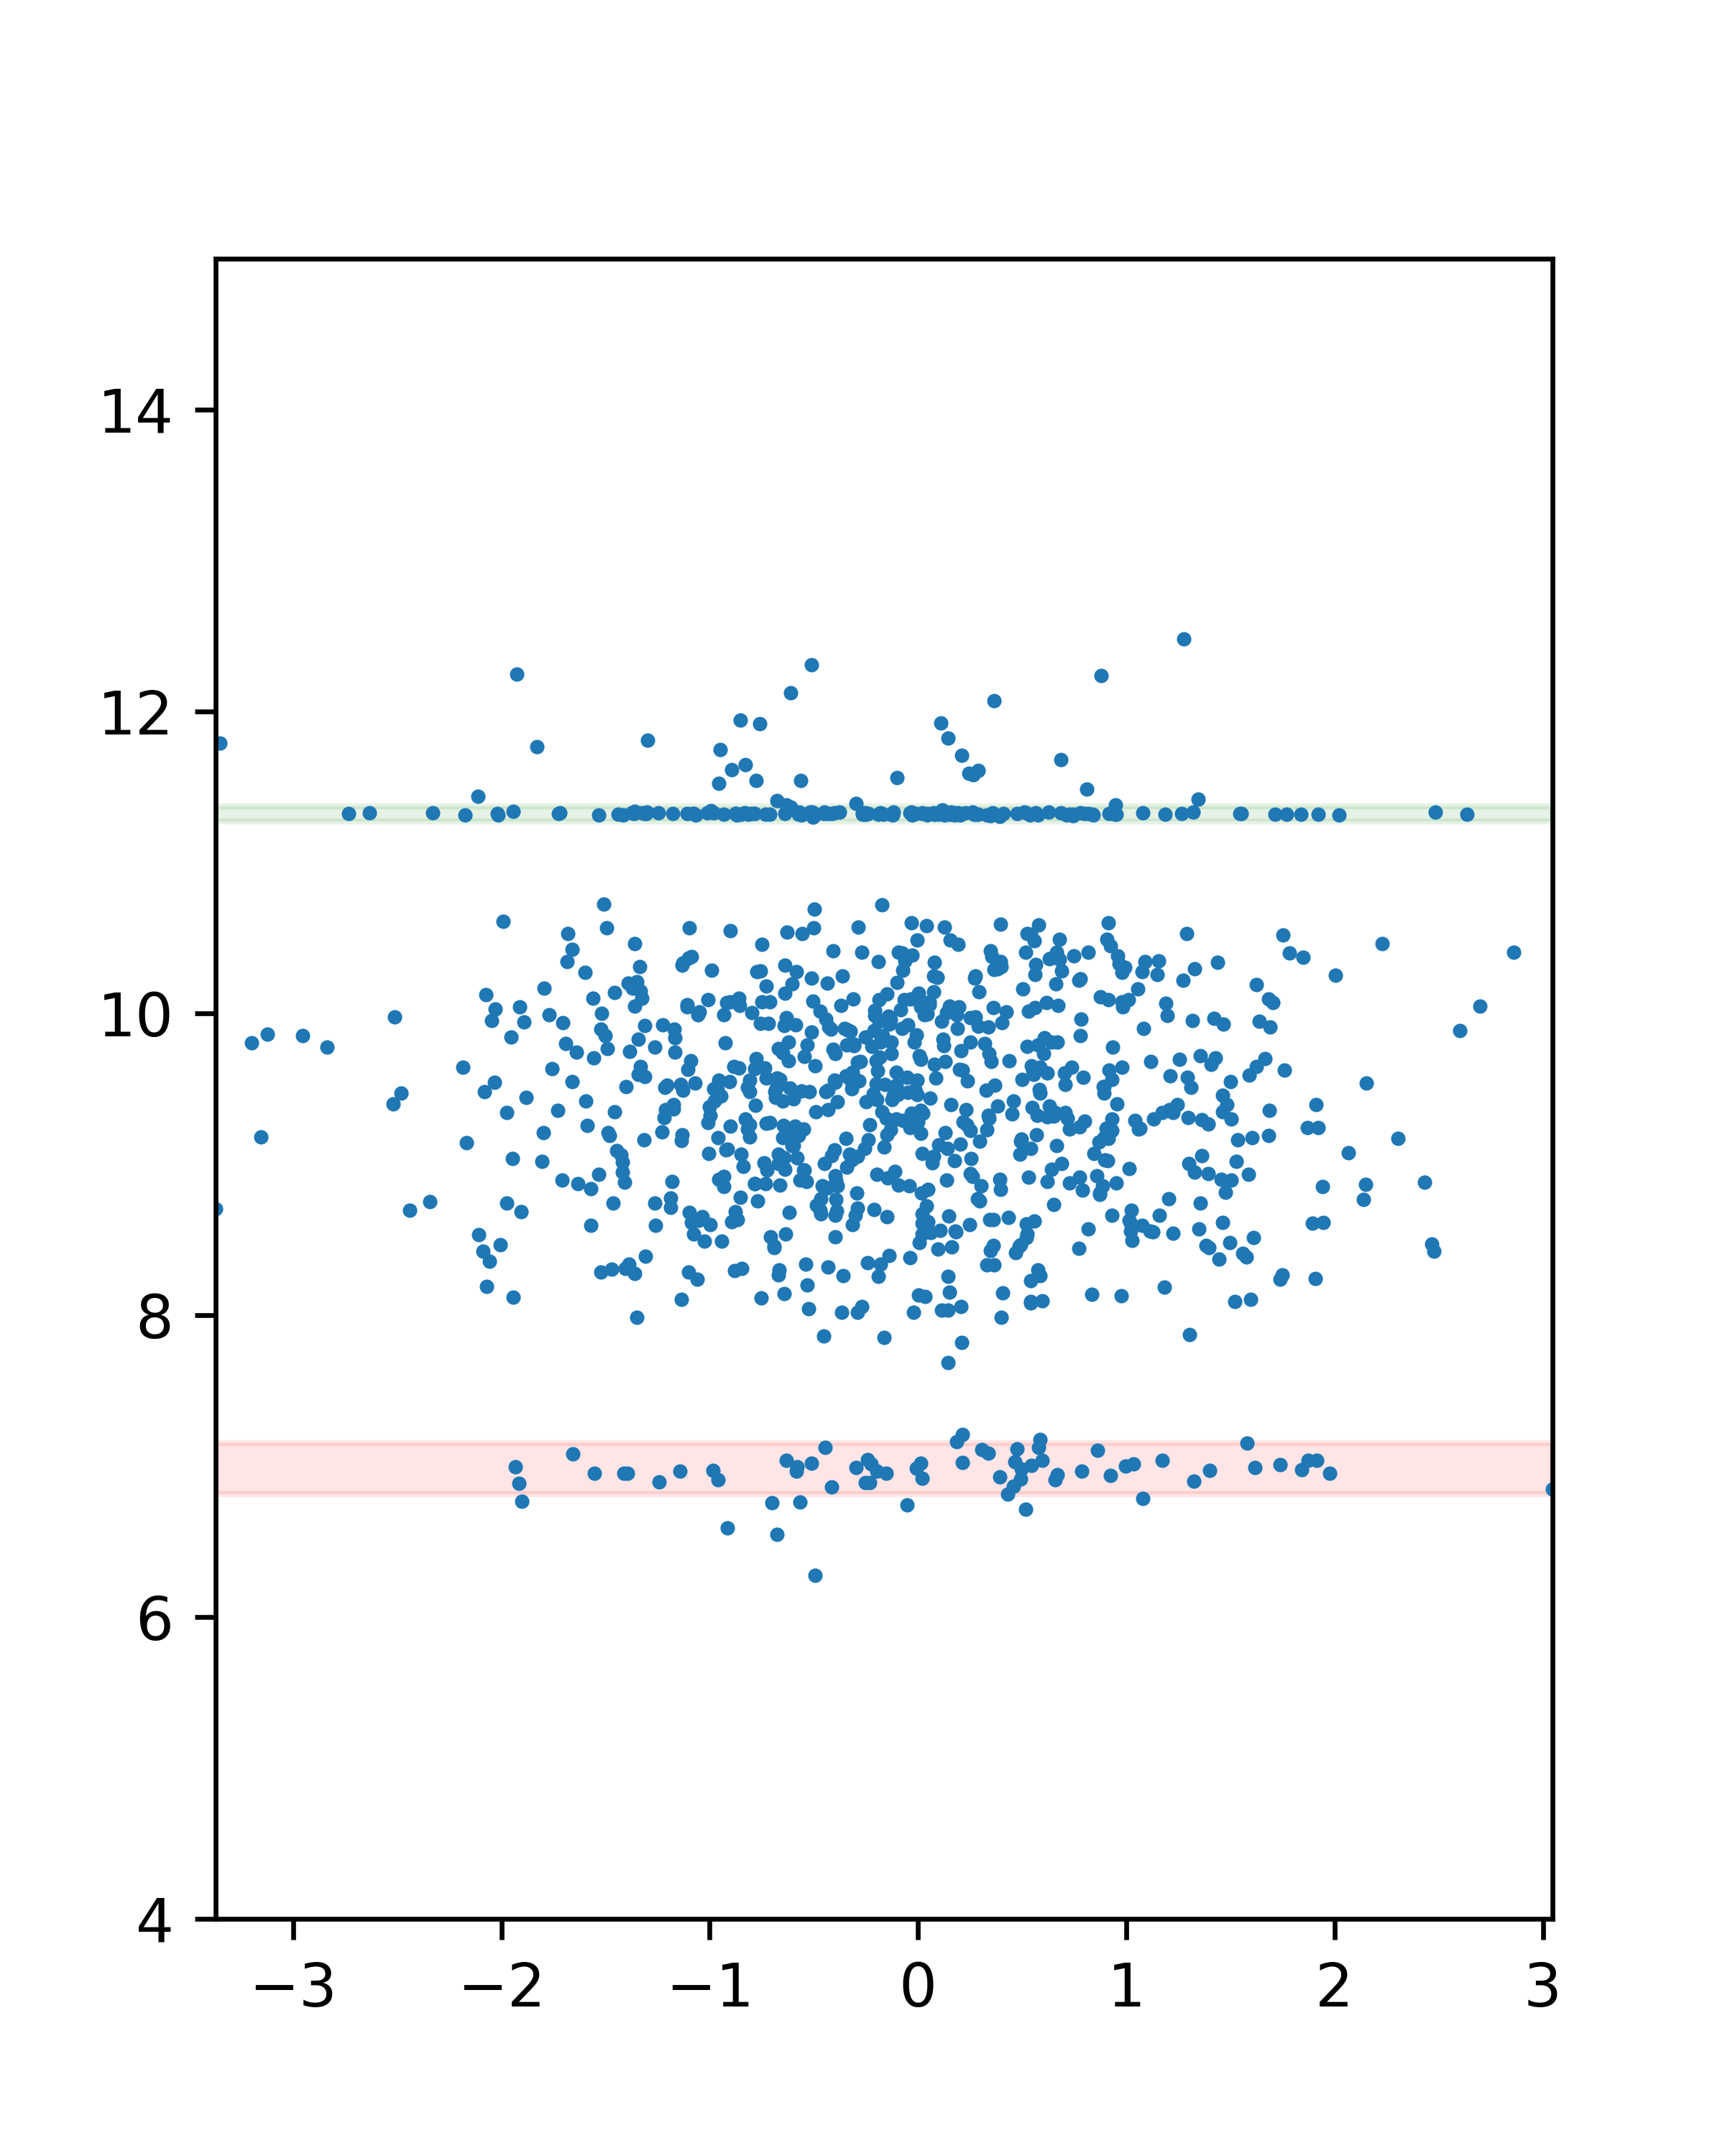
\includegraphics[width=\textwidth]{t_as}
  \end{columns}
\end{frame}

\begin{frame}{Optimal arrival time samples}
  As can be seen here, the zones in which early and late arrivals occour depend on where the steepness of the travel time function becomes high enough.
  \begin{center}
    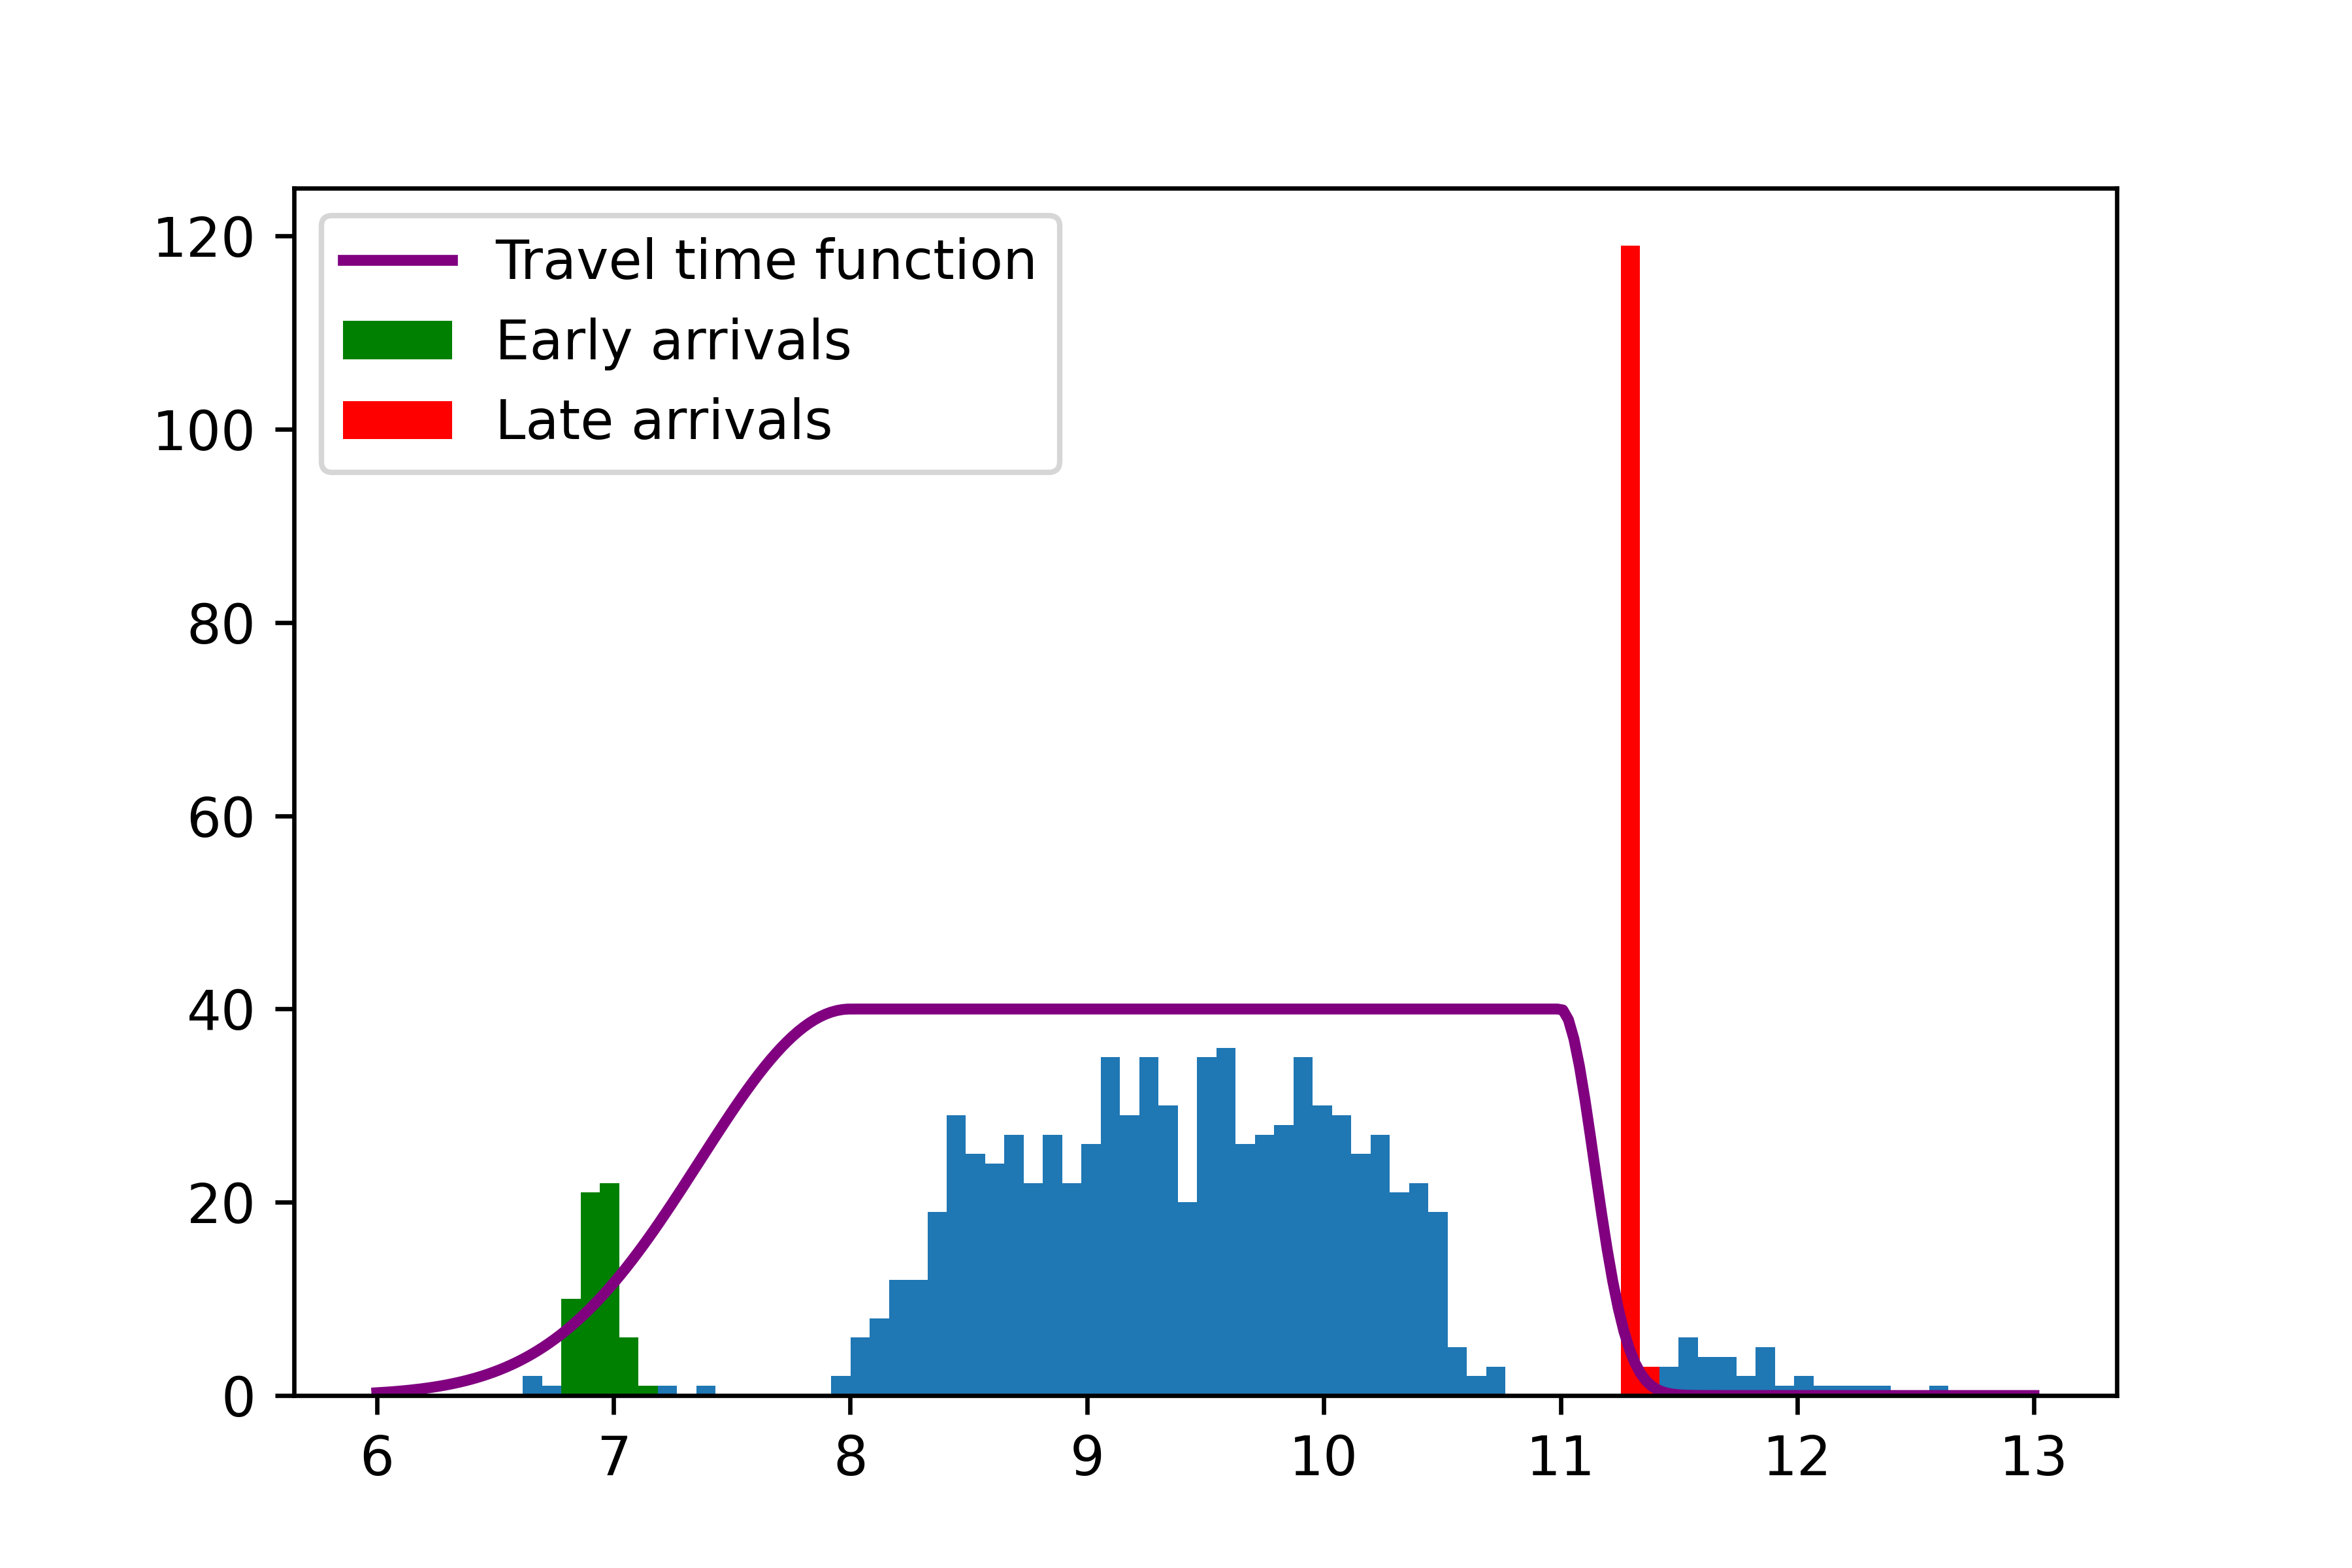
\includegraphics[width=\textwidth]{t_as_bins_tt}
  \end{center}
\end{frame}

\begin{frame}{Methodology}
  Our goal is thus finding, from the data about actual arrival times, the most likely values for the mean and variances of the parameters \(\beta\) and \(\gamma\), on top of mean and variance for the desired arrival time \(t^*\).

  This was done by modelling the actual likelihood of each data point for a given parameter set
  \begin{equation*}
    \mathcal{L}(\theta\ \vert\ T_a = t_a) =
  f_{T_a; \theta}(t_a)
  \end{equation*}
  where \(f_{T_a; \theta}\) is the probability density function for the random variable \(T_a\),
  which describes the resulting optimal arrival time (namely, the one depicted in the plots above), given the parameters \(\theta\), where
  \[\theta = (\mu_\beta, \mu_\gamma, \mu_t, \sigma, \sigma_t)\]
  
  Once the likelihood function is built, running an optimizer on the total likelihood of the dataset retrieves the true parameters for a given dataset.
\end{frame}

\begin{frame}{Building the likelihood function}
  To build the likelihood function, each point is assigned a probability of being an early, late or on time arrival.

  This is done by taking advantage of the key observation that early and late arrivals only occur when the desired arrival time \(t^*\) falls in certain zones defined by the parameters \(\beta\) and \(\gamma\), namely the shaded zones in the plot below

  \begin{center}
    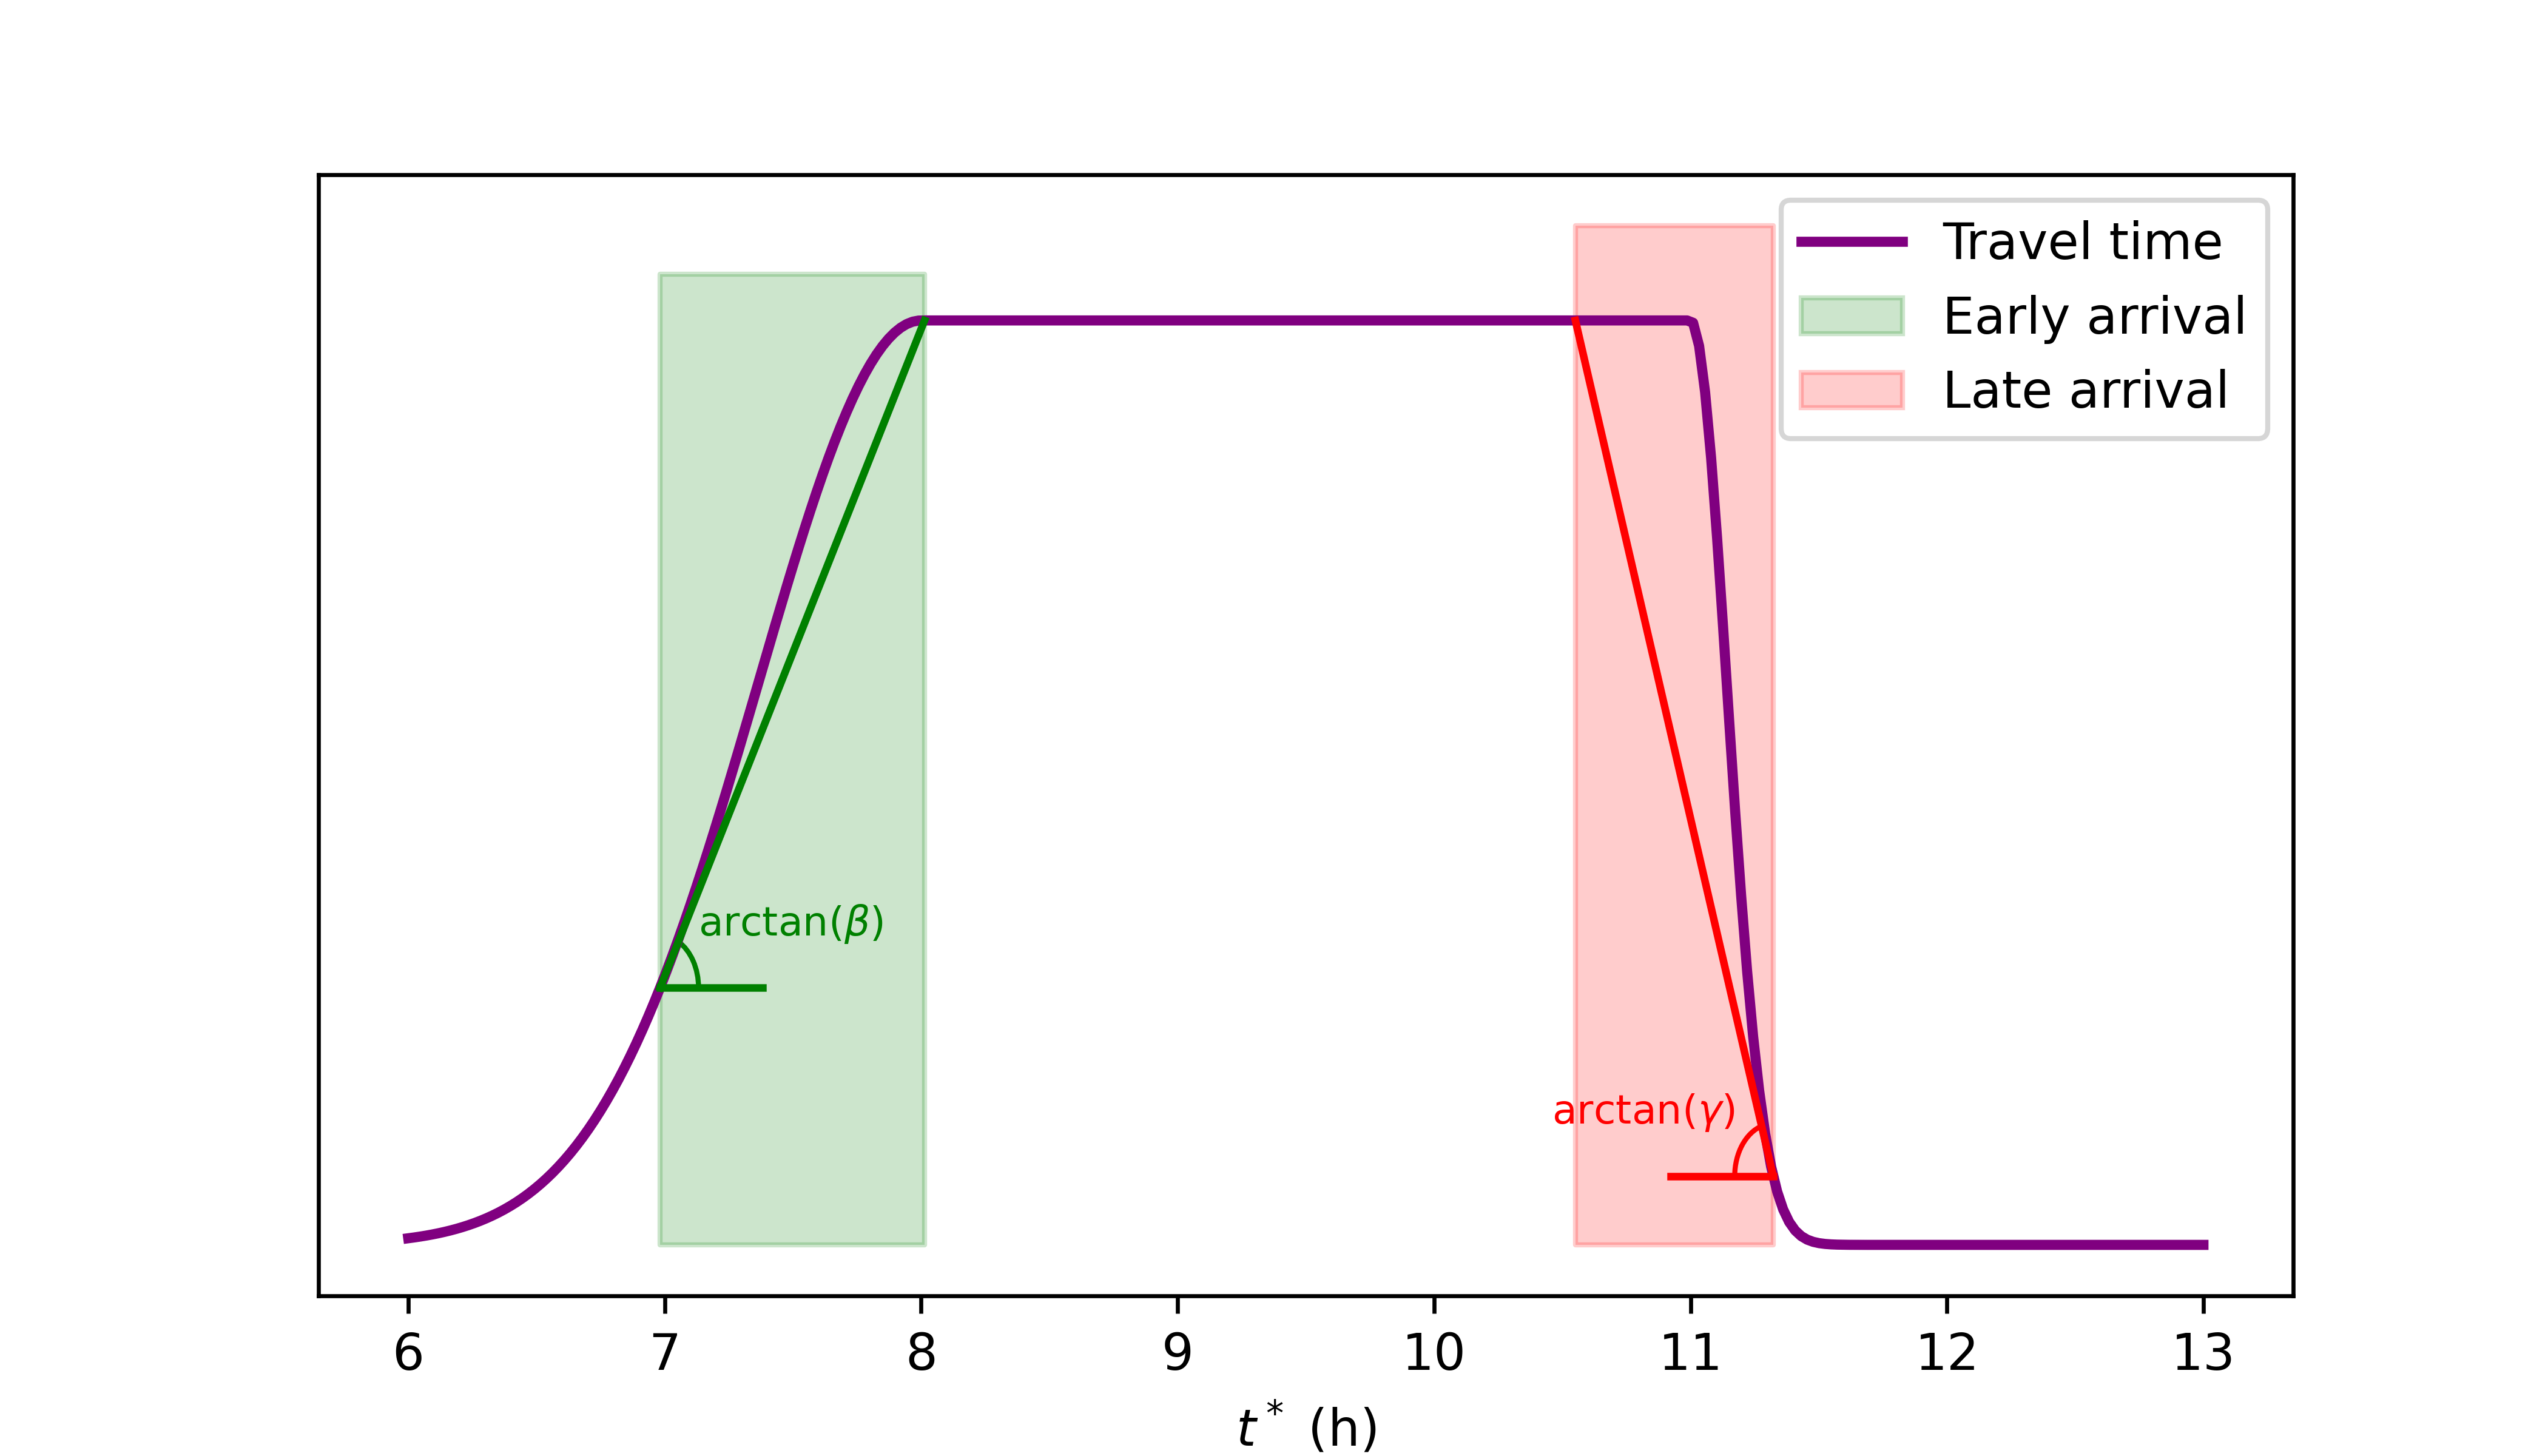
\includegraphics[width=.9\textwidth]{tt_early_late}
  \end{center}
\end{frame}

\begin{frame}{Building the likelihood function}
  This observation allows us to define a likelihood function:
  as can be seen below, given the actual parameters the empirical distribution arising from sampling data and directly minimizing the cost function \(C(t_a)\) is well described by our likelihood function

  \begin{center}
    \alt<2>{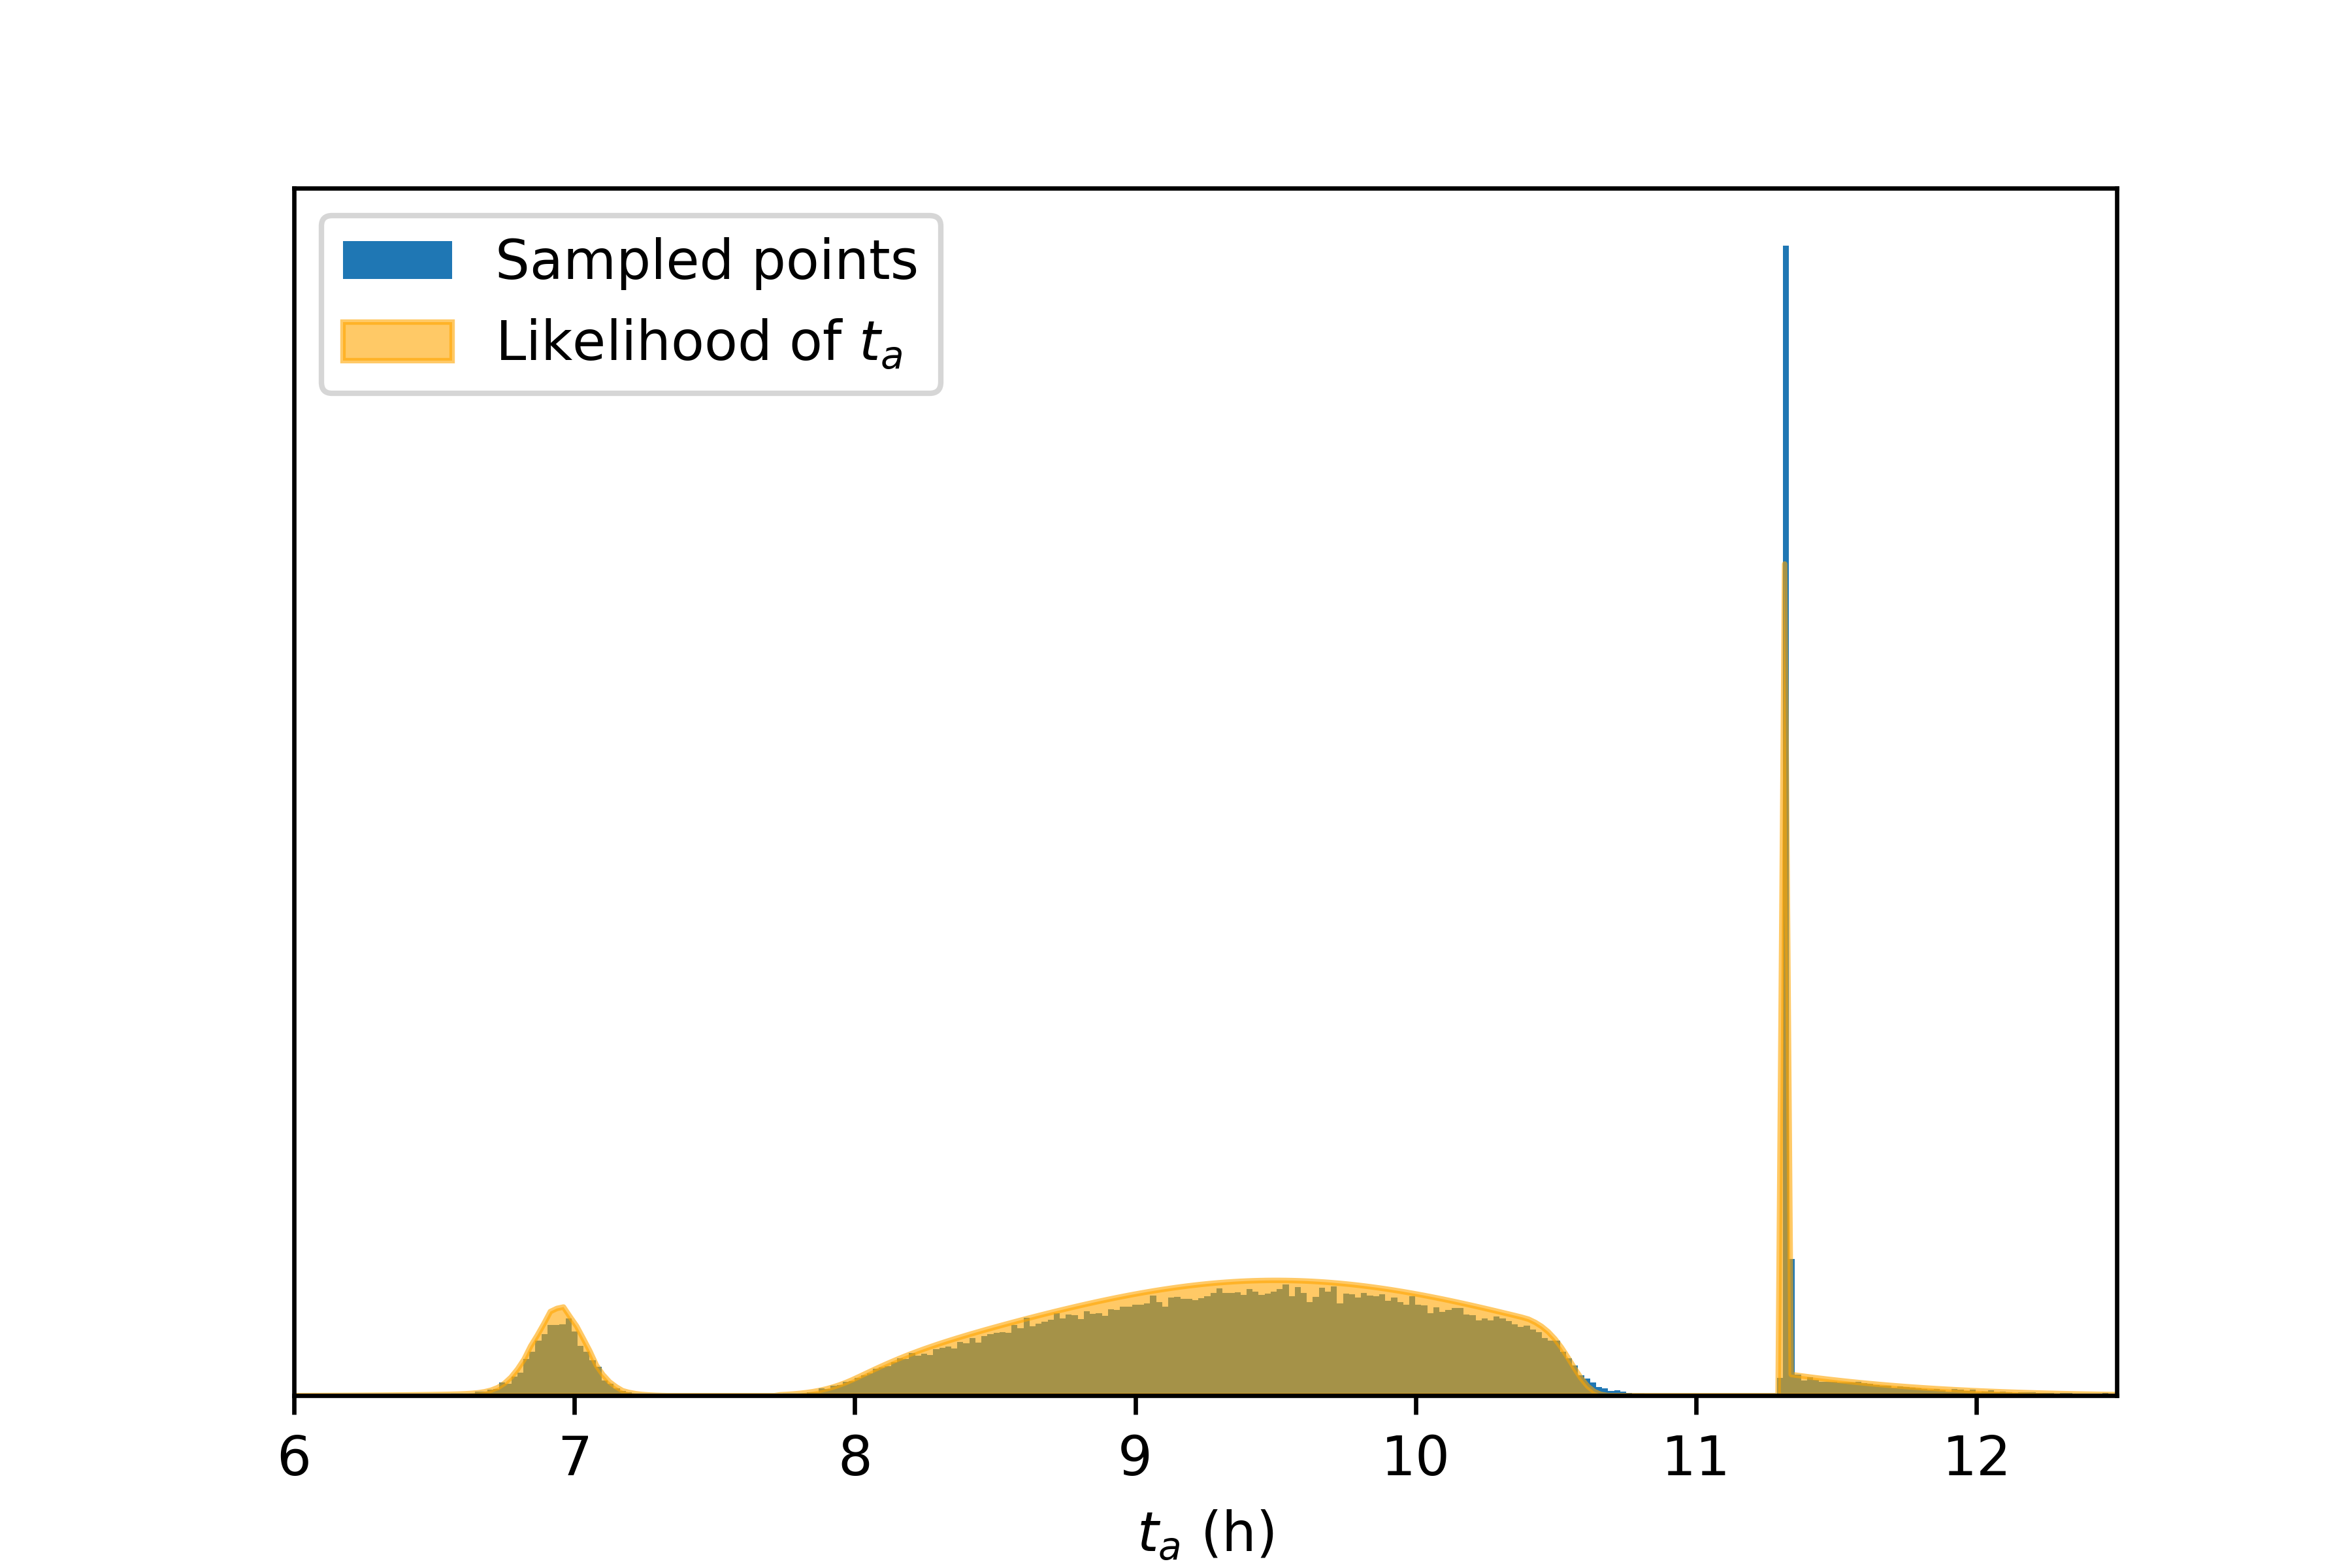
\includegraphics[width=.9\textwidth]{hist_ll}}{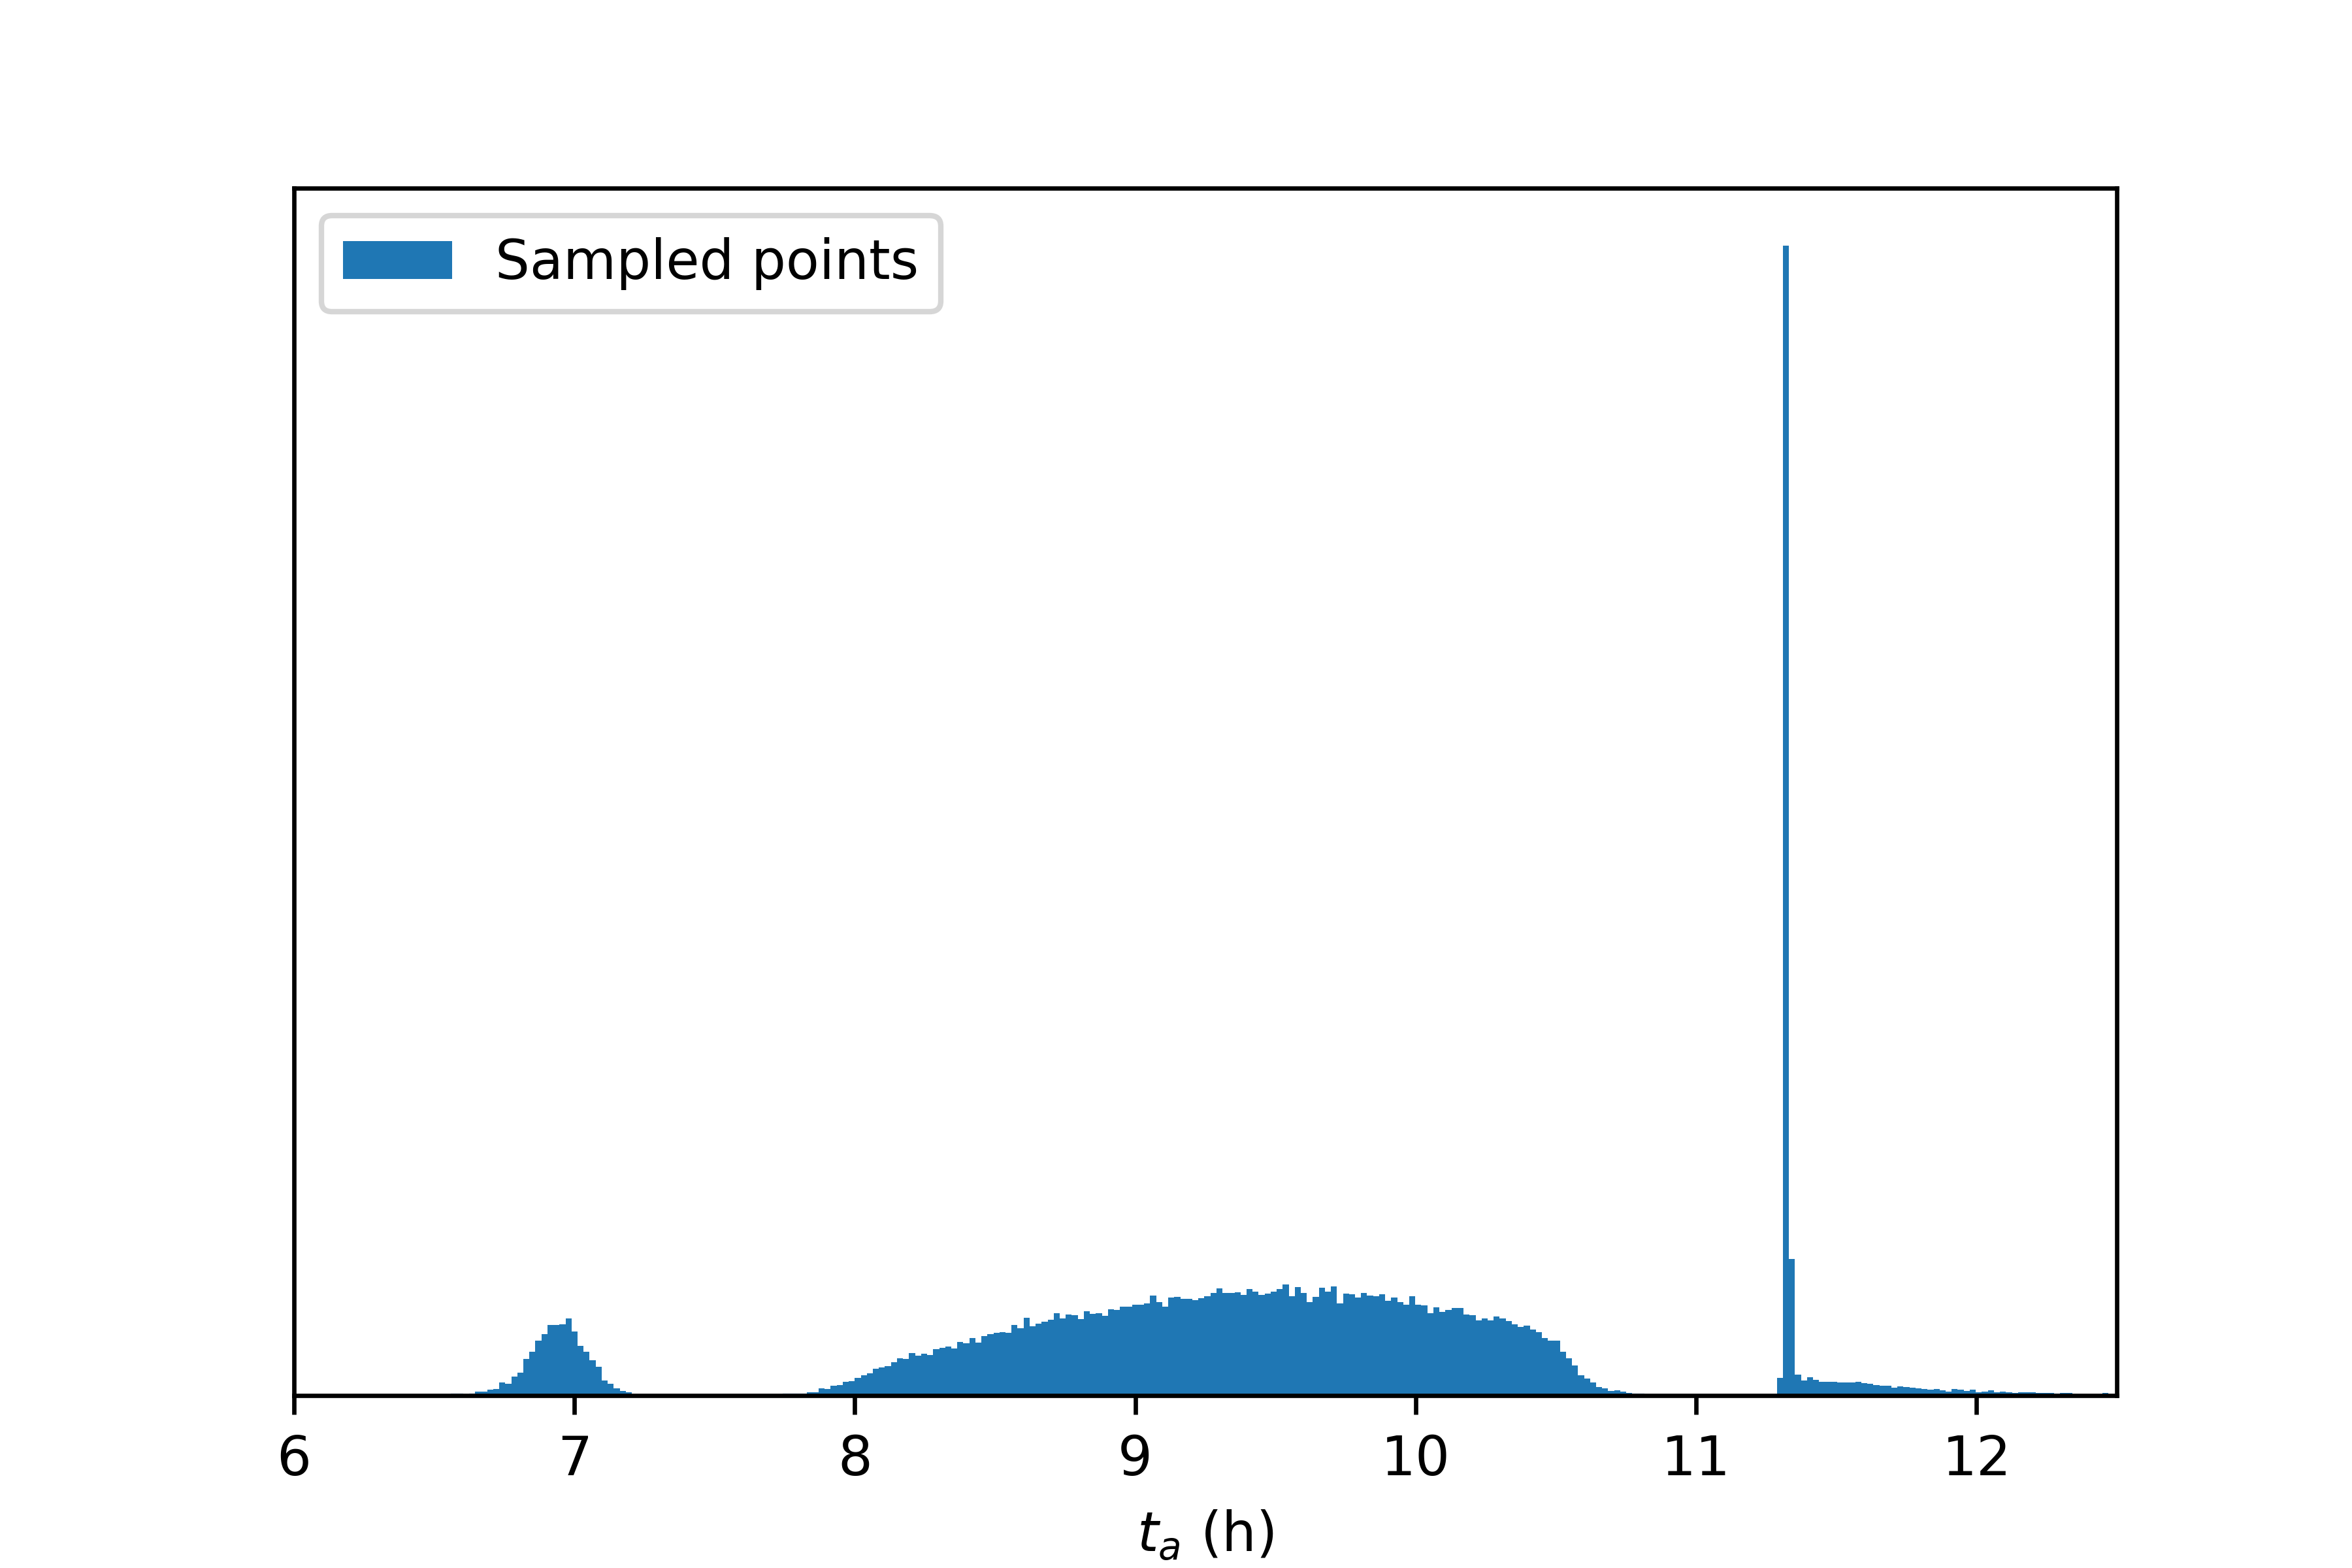
\includegraphics[width=.9\textwidth]{hist_no_ll}}
  \end{center}
\end{frame}

\begin{frame}{Computation of the likelihood function}
  Computing the likelihood \(\mathcal{L}(\mu_\beta, \mu_\gamma, \mu_t, \sigma, \sigma_t\ \vert\ T_a = t_a)\) is computationally not trivial, since it requires to invert various functions and to compute different integrals.

  It was made possible by extensively using the python library JAX, which considerably sped up the calculations (by different orders of magnitude) and allowed us to have a fast enough likelihood function to be able to run an optimizer over it.

  Moreover, the library JAXopt  would allow us to run a Gradient Descent algorithm over the total likelihood.
  For problems with numerical stability, this approach is not fully developed yet, but will be explored in the future.
\end{frame}

\begin{frame}{Properties of the likelihood function}
  Given a dataset, the likelihood function is thus defined on a five-dimensional space.

  By evaluating it on a synthetic dataset, the original parameters can be known,
  and some 2-dimensional slices of the function can be plotted.

  By plotting the mean parameters \(\mu_\beta, \mu_\gamma\) (and freezing \(t^*, \sigma\) and \(\sigma_t\) to their known, true value) it can be seen how the likelihood is better behaved when the variance \(\sigma\) is not too low:
a low value for the variance could yield indeed a local minimum for a different value of the mean \(\mu_\gamma\).
  
\end{frame}

\begin{frame}{Changing the variance of the parameters \(\beta\), \(\gamma\)}
  \only<1>{When variances assume some moderate values,
    the likelihood function is well behaved, and the optimizers show no problems in converging:
    
    Here is the likelihood for variance \(\sigma = 0.3\)}

  \only<2>{On the other hand, extreme values for the variance lead to problematic likelihood functions:

    Here is the likelihood for variance \(\sigma = 0.03\)}

\only<-3>{

  \begin{center}
    \alt<-1>{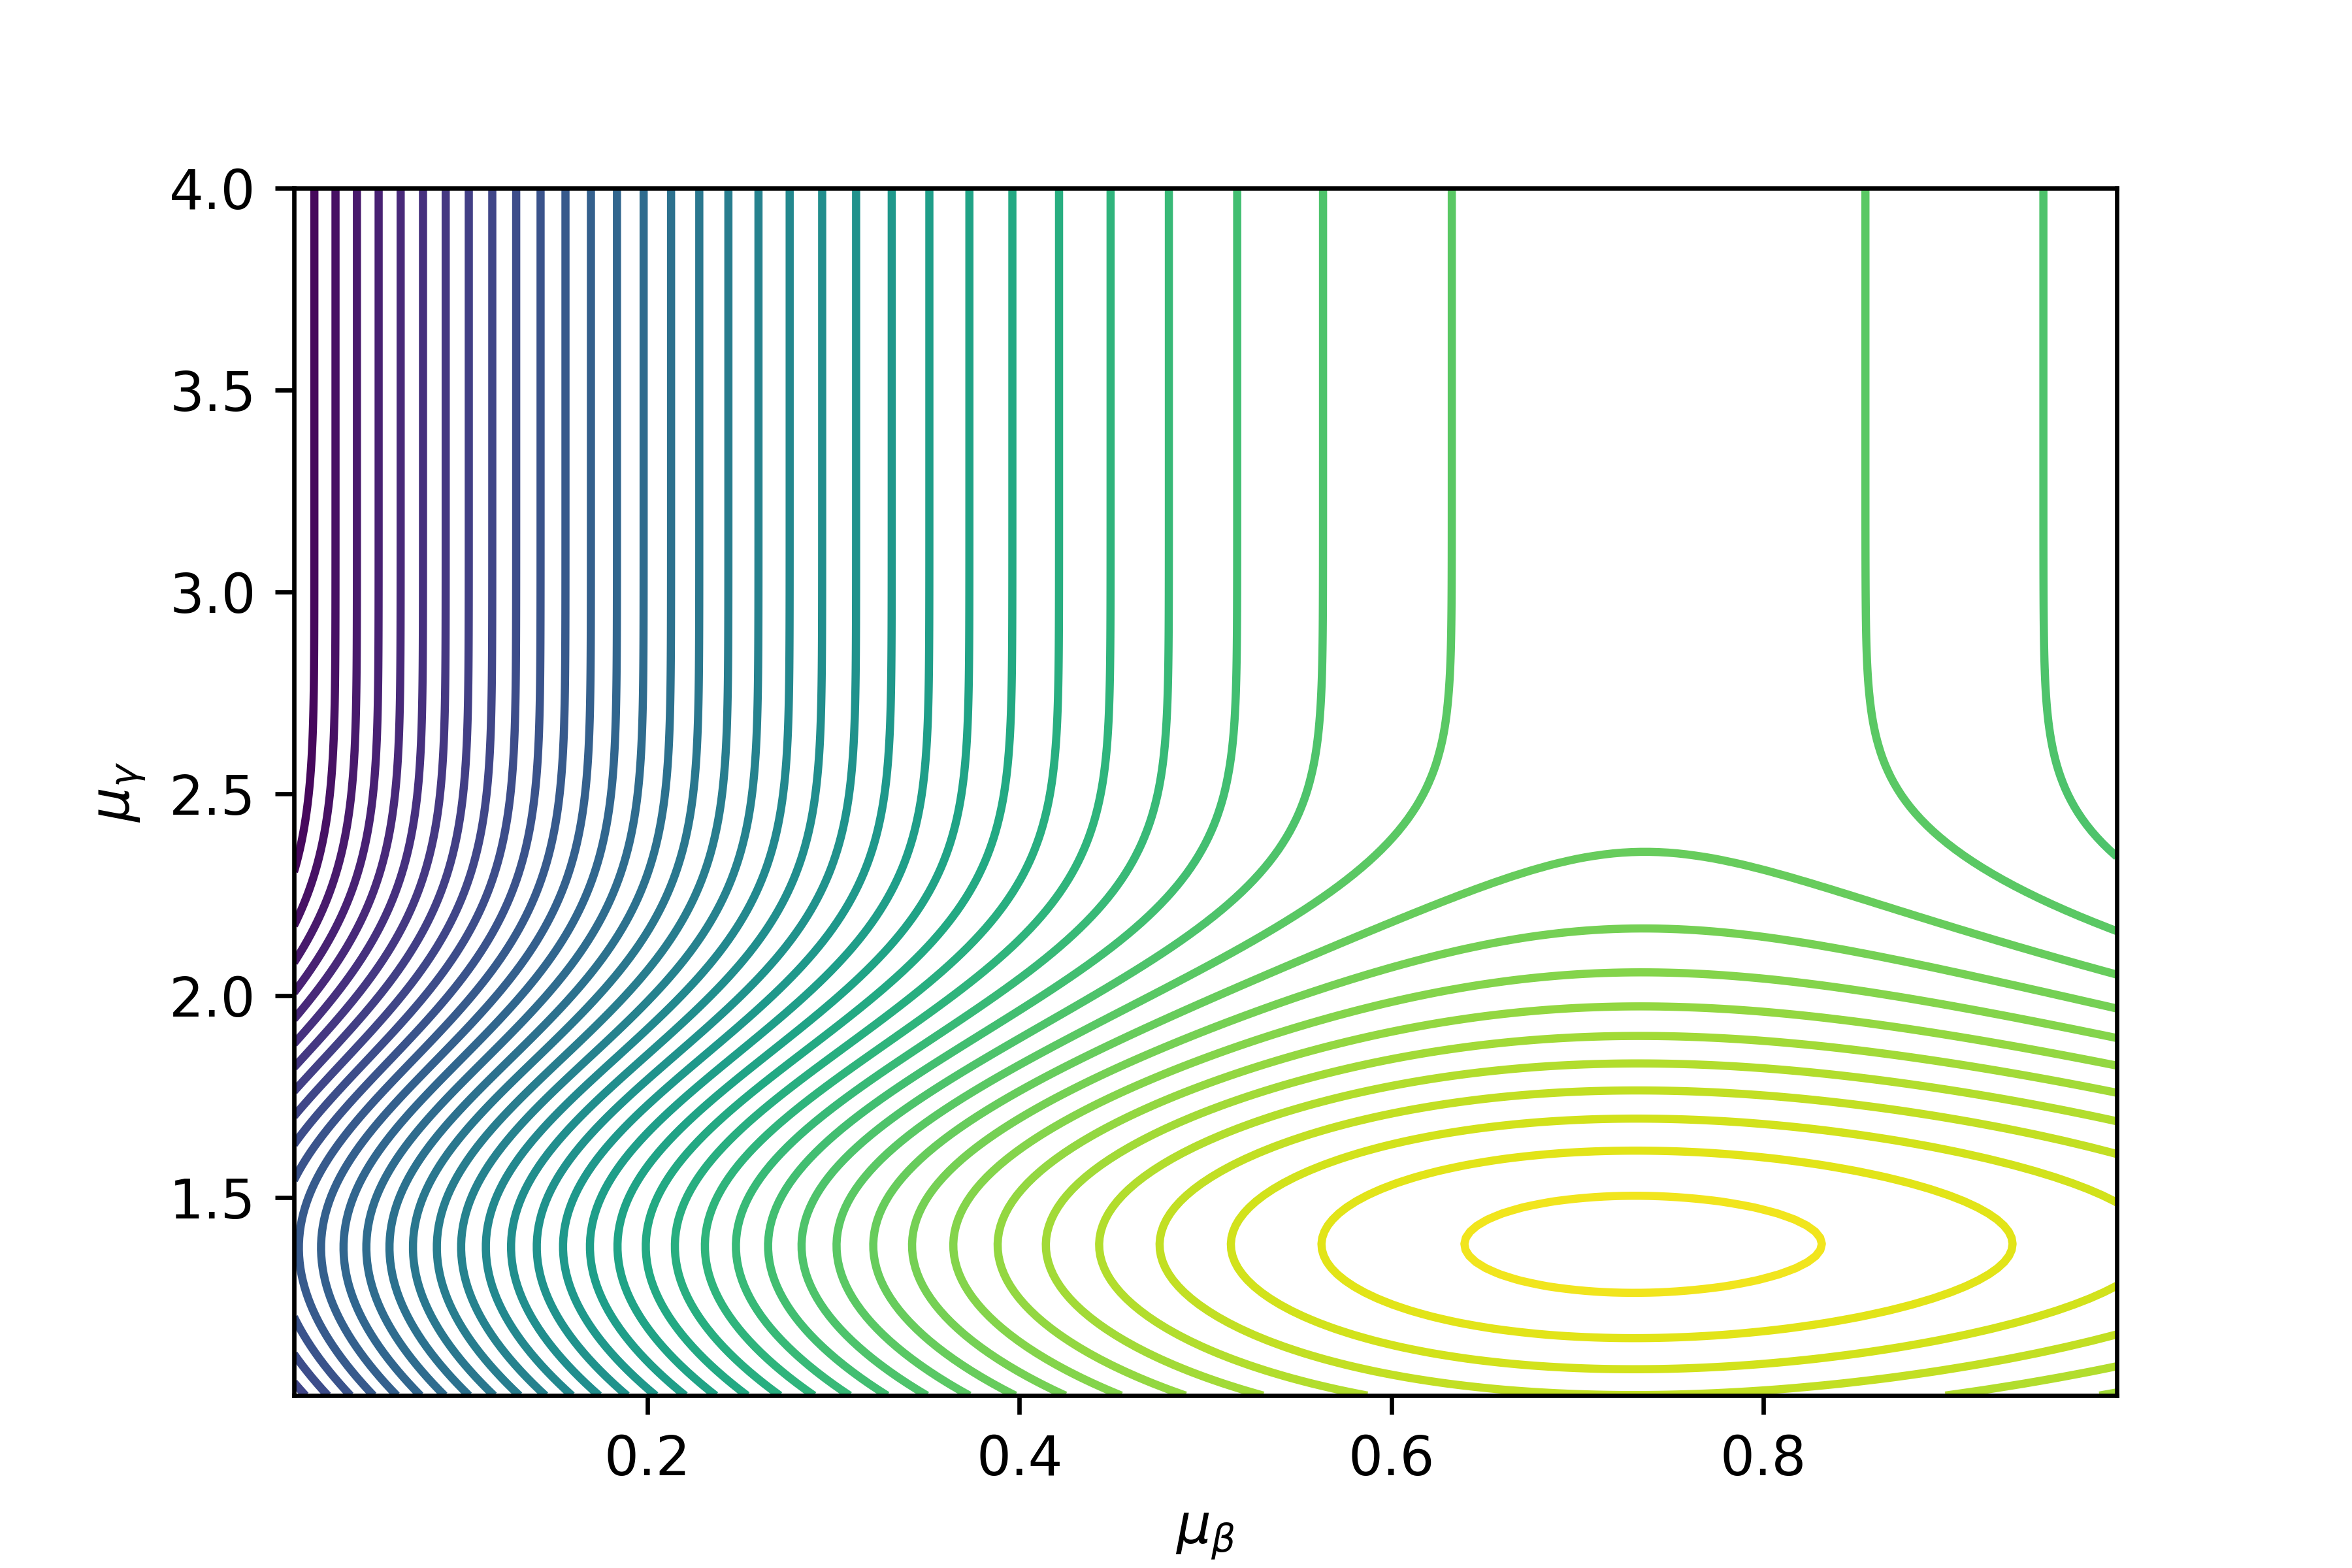
\includegraphics[width=.8\textwidth]{contour_beautiful}}{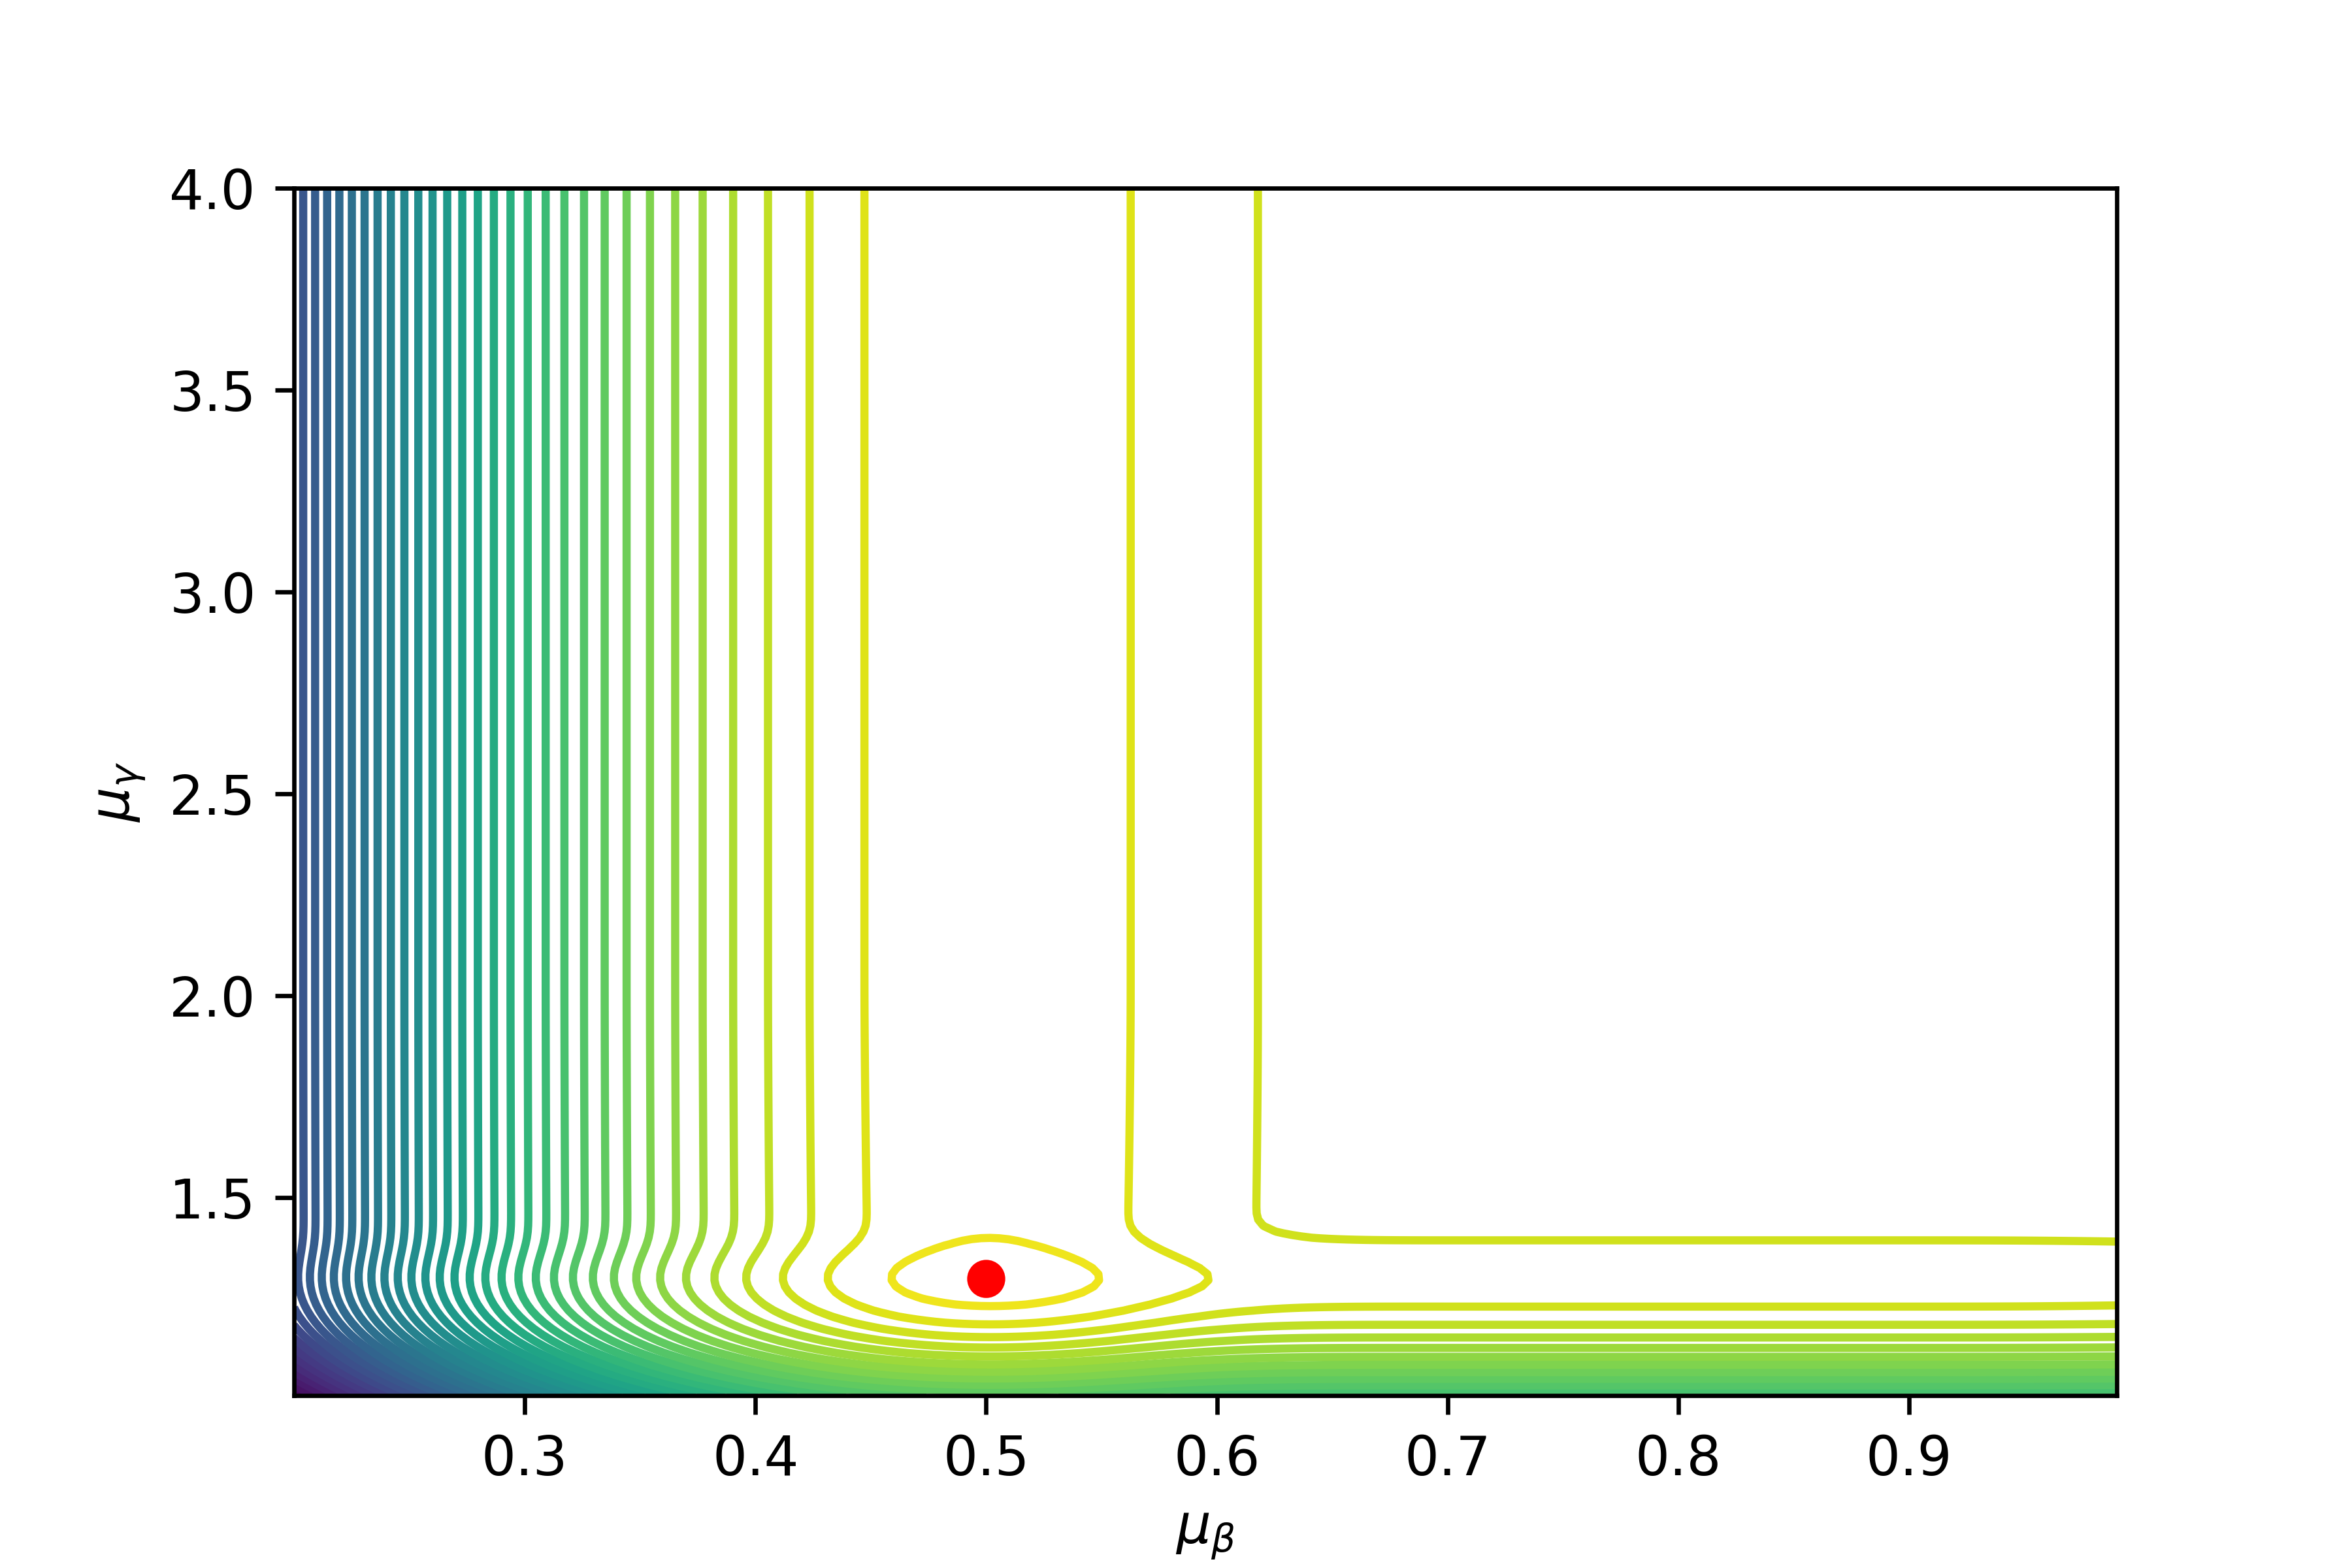
\includegraphics[width=.8\textwidth]{contour_ugly}}
  \end{center}
}
  \only<3>{
    It can be seen how the likelihood is almost constant in \(\mu_\gamma\), and thus problematic to optimize.

    There actually is a sharp minimum in the real parameters, but it is so sharp that it is difficult to see, and often smaller than the grid used for plotting the contour.
  }
  \only<4>{
    
    Lastly, with high variances the minimum becomes extremely flat,
    yielding another situation in which the optimizers are not very precise.
    }
\end{frame}

\begin{frame}{Reprocessing the real travel time data}
  \only<1>{
    Many travel time data provide actually the instantaneous
  travel time, which is calculated by the real-time travel speed at different locations of the
  route. However, our model requires the experienced travel time instead of the instantaneous
  travel time. Actually, we expect that the experienced travel time will increase faster than
  the instantaneous travel time.
}
\only<2>{
  For computing the actual travel time, we suppose that the bottleneck has fixed length \(d^p\),
and that in each moment the instantaneous travel time \(v(t)\) is constant along it.
The length of the bottleneck will thus be
}
\only<2->{
  \begin{equation}
    \label{eq:len_bottleneck}
    d^p = \int_{t_i}^{t_f}v(t) dt
  \end{equation}
}
\only<3>{
  Suppose thus \(v(t)\) has primitive \(V(t)\), such that

\begin{equation}
  \label{eq:primitive}
  \int_{t_i}^{t_f}v(t) dt = V(t_f) - V(t_i)
\end{equation}

The equation above equation becomes trivially

\begin{align*}
  d^p & = V(t_f) - V(t_i) \\
  t_i & = V^{-1}(V(t_f) - d^p)
\end{align*}
and the travel time can thus be expressed in function of \(t_f\):
\begin{align*}
  \begin{split}
    \label{eq:travel_time}
    tt(t_f) & = t_i - t_f \\
    & = V^{-1}(V(t_f) - d^p) - t_f
  \end{split}
\end{align*}
}
\end{frame}

\begin{frame}{Reprocessing the real travel time data}
  In the case in which the instantaneous travel time increase linearly, its primitive is easy to compute and to invert:

\begin{align*}
  v(t) & = \bar{v}t \\
  V(t) & = \frac{\bar{v}}{2}t^2 \\
  V^{-1}(x) & = \sqrt{\frac{2x}{\bar{v}}}
\end{align*}
and thus,
\begin{align*}
  tt(t_f) & = \sqrt{\frac{2}{\bar{v}}\left(\frac{\bar{v}}{2}t_f^2 - d^p\right)} - t_f \\
  & = \sqrt{t_f^2 - \frac{2}{\bar{v}}d^p} - t_f
\end{align*}

\end{frame}

\begin{frame}{Numerically reprocessing the real travel time data}
  Numerically, it may be impossible (or very inconvenient) to find the actual primitive \(V(t)\).

An approach that can be taken (especially when the travel time function is just a discrete set of values) is to directly approximate the integral.
This can be done by progressively increasing the domain of integration (where the integration is discrete, approximated with trapezoids),
until the integral becomes larger than the bottleneck length \(d^p\).

The figure in the following slide shows the result of this process.
\end{frame}

\begin{frame}
\begin{figure}
  \centering
  \makebox[\textwidth][c]{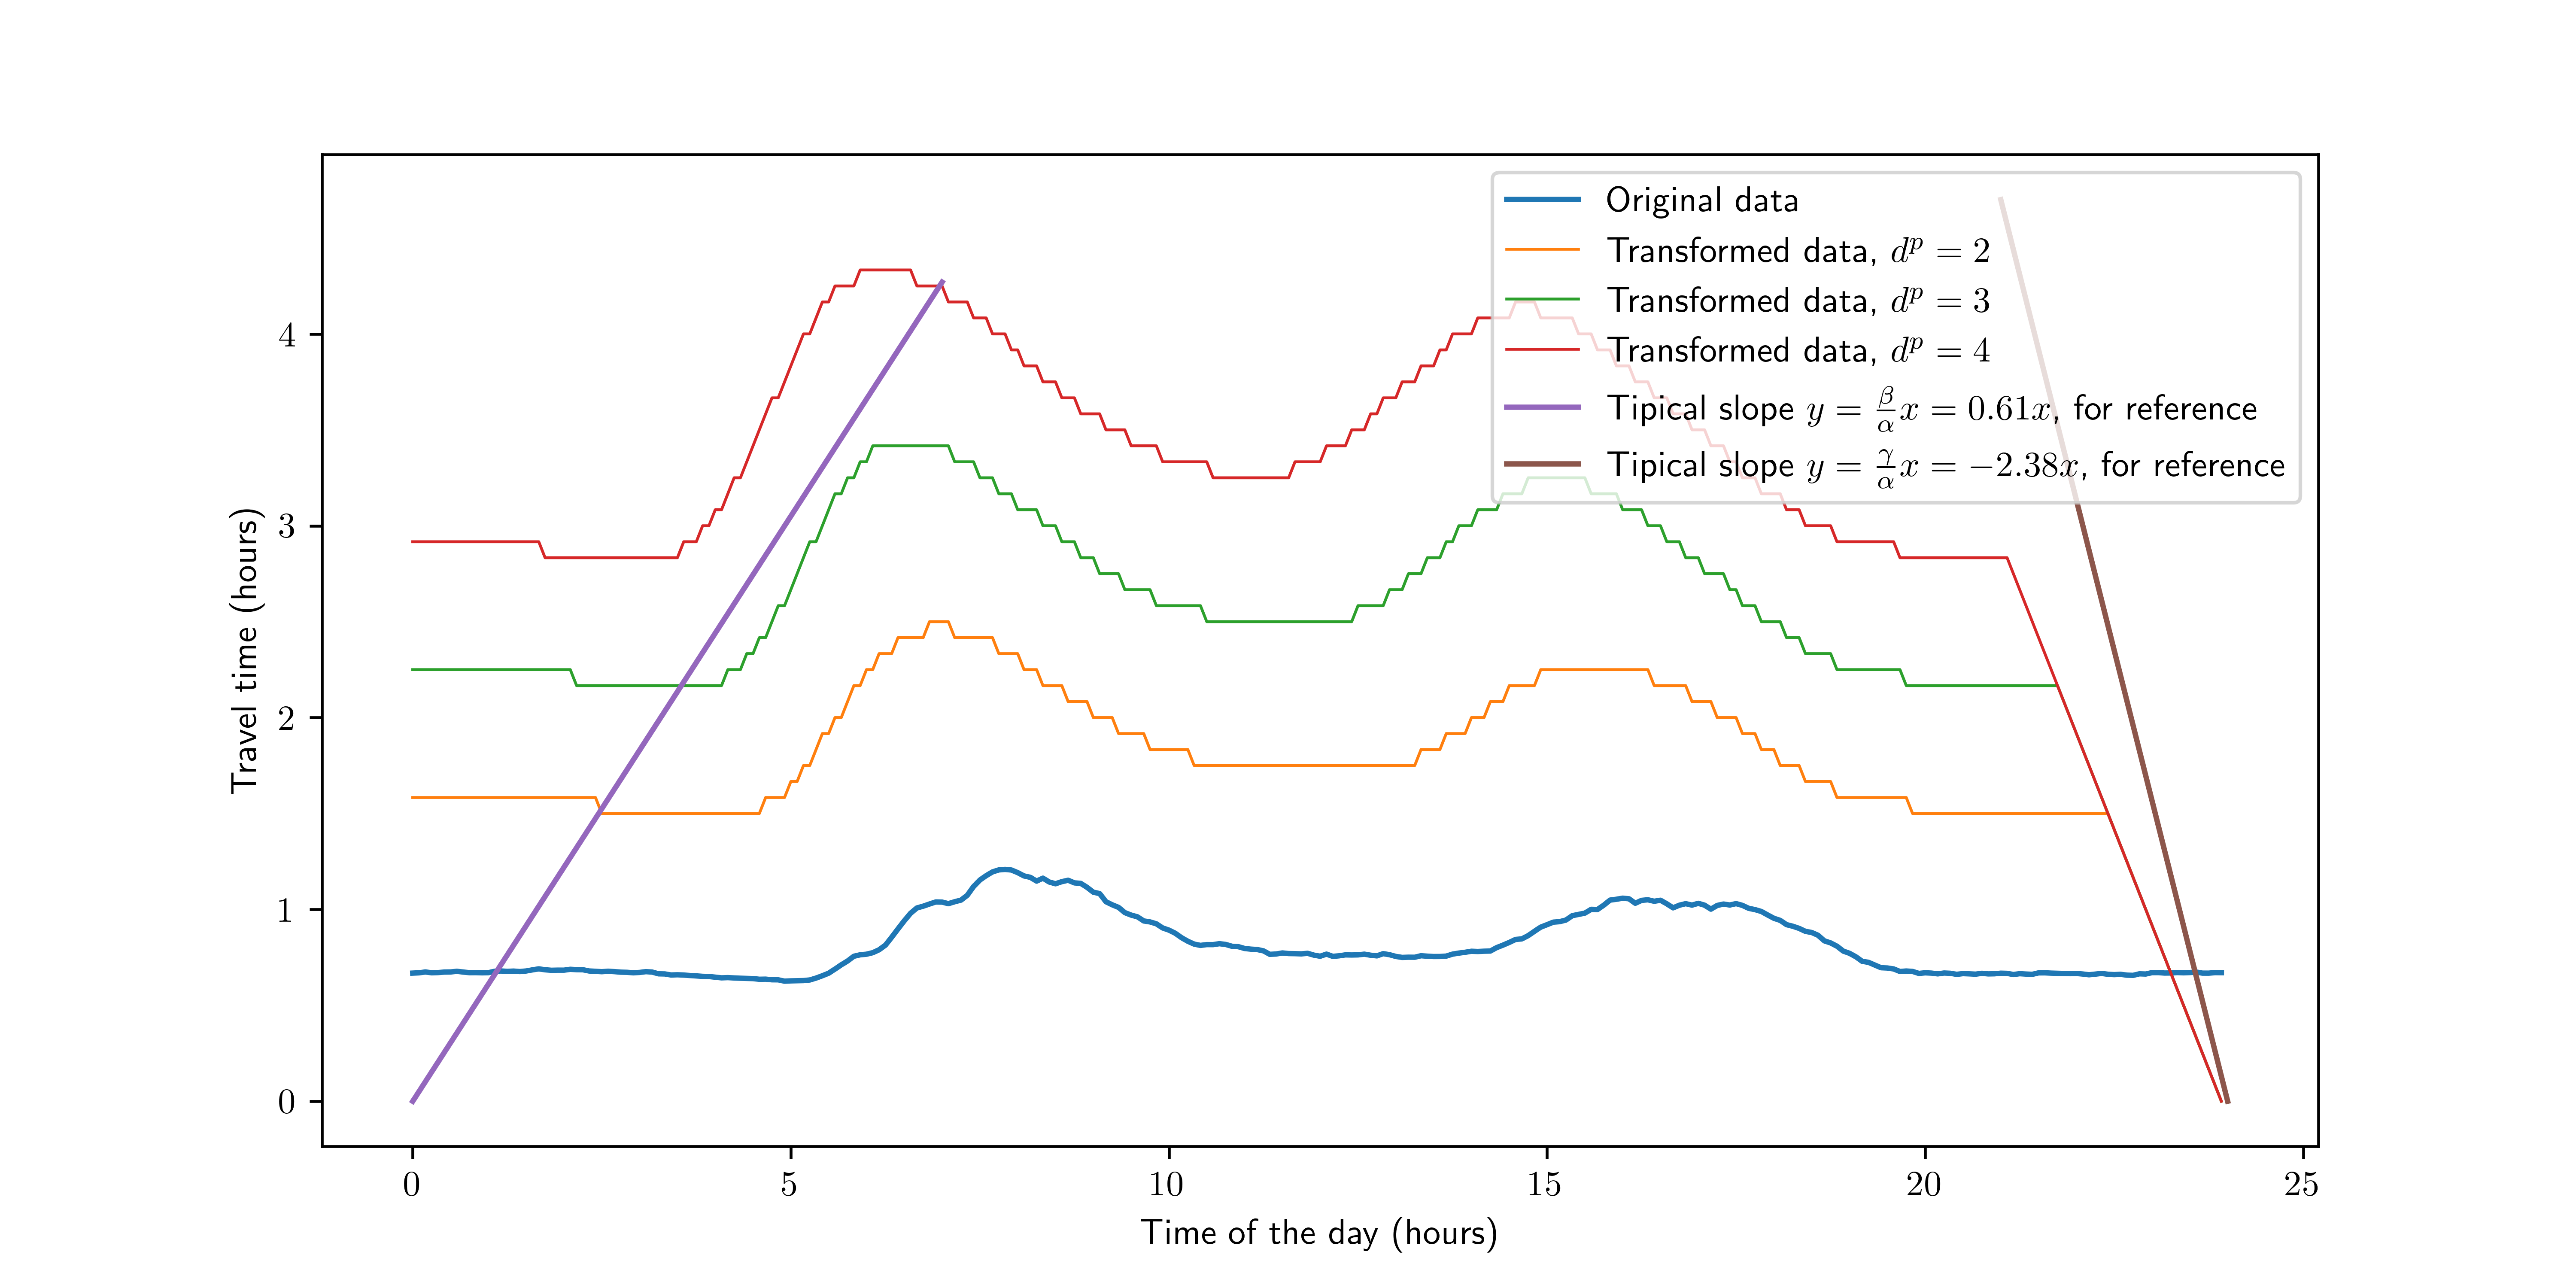
\includegraphics[width=1.3\textwidth]{img/transforming_data}}
  \caption{Transformed data, for different values of the bottleneck length $d^p$. The lines whose steepness yields late and early arrivals are shown for reference, in order to be able to appreciate the increasing steepness.}
  \label{fig:modifying_data}
\end{figure}


\end{frame}

\end{document}

%%% Local Variables:
%%% mode: LaTeX
%%% TeX-master: t
%%% End:
